% Built with: make paper   (tectonic morphogen.tex)
%
% Every number and every figure in this document is produced by tools/figures.c,
% which links against exactly the same simulation core that runs in the browser.
% There is no separate "figure code" that could drift away from the thing being
% described: if a plot here is wrong, the simulation is wrong.
\documentclass[11pt,a4paper]{article}

\usepackage[T1]{fontenc}
\usepackage[utf8]{inputenc}
\usepackage{lmodern}
\usepackage[margin=2.6cm]{geometry}
\usepackage{amsmath}
\usepackage{graphicx}
\usepackage{booktabs}
\usepackage{siunitx}
\usepackage{caption}
\usepackage{subcaption}
\usepackage{pgfplots}
\usepackage{pgfplotstable}
\usepackage{microtype}
\usepackage[hidelinks]{hyperref}
\usepackage{xcolor}

\pgfplotsset{compat=1.18}
\definecolor{ink}{HTML}{2B2B2B}
\definecolor{papergrey}{HTML}{F2F1E8}
\definecolor{accent}{HTML}{4A7FCB}
\definecolor{warm}{HTML}{C0472F}

\pgfplotsset{
  every axis/.append style={
    axis line style={ink!55, line width=0.4pt},
    tick label style={font=\scriptsize, color=ink!75},
    label style={font=\small, color=ink},
    title style={font=\small\bfseries, color=ink},
    grid style={ink!12, line width=0.3pt},
    legend style={font=\scriptsize, draw=ink!25, fill=white, rounded corners=1pt},
    axis background/.style={fill=white},
    width=7.6cm, height=5.2cm,
  },
}

\captionsetup{font=small, labelfont=bf}
\setlength{\parskip}{0.35em}

\title{\textbf{morphogen}: a browser-native laboratory for cellular automata\\
       and agent-based models}
\author{Enes \"Oz\\[2pt]
        \small\texttt{https://github.com/en970/morphogen}\\
        \small\texttt{https://en970.github.io/morphogen}}
\date{July 2026}

\begin{document}
\maketitle

\begin{abstract}
\noindent
Cellular automata are usually presented on the web as pictures. This is a
laboratory: ten models drawn from the primary literature, with the parameters
their authors used, simulation cores written in C and compiled to WebAssembly,
and quantitative observables computed and plotted while the model runs. Every run
is a pure function of a seed and a parameter vector, both of which live in the
address bar, so a link reproduces a run cell for cell rather than merely
depicting one. The models are not validated against themselves; they are
validated against numbers other people measured. A nutrient-starved colony
box-counts to a fractal dimension approaching the Witten--Sander value of
\num{1.71}; the same colony, fed, fills in as a disc of dimension \num{2.0}. Rule
90 from a single live cell reproduces the Sierpi\'{n}ski triangle at
$D=\log 3/\log 2=\num{1.585}$. Sugarscape drives a Gini coefficient from equal
endowments to $\approx\!\num{0.4}$. Schelling's households, each content to be
outnumbered two to one, segregate a city to $\approx\!\num{0.77}$ against a
chance baseline of $\num{0.50}$. These are assertions in a test suite that runs on
every commit. We also report what did not work, and why the failures were
instructive: in particular, an early version of the colony model produced a
diffuse cloud of wandering cells that box-counted to a perfectly respectable
$D\approx\num{1.71}$ while being, physically, nothing like a colony --- a
cautionary result about the sufficiency of a single scalar observable.
\end{abstract}

\section{Introduction}

The interesting thing about a cellular automaton is not that a simple rule can
produce a complicated picture. It is that a rule with no notion of the global
object it is building --- no representation of a colony, a spiral, a city, or a
species --- nevertheless builds one, and builds a specific one, whose properties
can be measured and compared against a laboratory.

That comparison is the part that is usually missing. There is no shortage of
Game-of-Life implementations on the web, and several of them are beautiful. Very
few of them measure anything, and almost none of them let you take a
configuration you found and hand it to somebody else exactly as you found it.
Without measurement, a simulation is an illustration of a claim rather than a
test of one; without reproducibility, it is not an instrument at all.

This paper describes \textbf{morphogen}, which attempts both. It contains ten
models, chosen so that they form a single argument rather than a menu: rules,
then chaos, then chemistry, then colonies, then ecosystems, then societies, then
criticality. The question they are arranged around is deliberately naive, and it
is the one that makes cellular automata worth taking seriously in the first
place:

\begin{quote}
\emph{How does something alive --- a bacterial colony, an ecosystem, a society
--- find food, survive, adapt, and organise itself, when nothing in it can see
further than its own neighbours?}
\end{quote}

\paragraph{Contributions.}
\begin{enumerate}\setlength{\itemsep}{2pt}
  \item A portable C99 simulation core with a common model interface, compiled
    both natively (for testing and profiling) and to WebAssembly (for the
    browser), with an observable bus that every model streams into.
  \item Bit-exact reproducibility: a seed and a parameter vector determine a run
    completely, and both are carried in the URL fragment.
  \item Validation against the primary literature, as executable assertions
    (\S\ref{sec:validation}), rather than against the implementation's own prior
    output.
  \item A rendering method that treats the display as a printing press rather
    than a screen: each field is a halftone separation at its own screen angle
    (\S\ref{sec:render}).
  \item Negative results (\S\ref{sec:negative}), including one that we think is
    generally useful: a fractal dimension in the right range is weak evidence
    that a growth model is right.
\end{enumerate}

\section{Architecture}

\subsection{The core is not a web project}

\texttt{src/core/} is portable C99 and has no dependency on Emscripten, on
JavaScript, or on the existence of a browser. It compiles with the system
compiler and runs on the command line. This is the single most useful structural
decision in the project: it means the models can be unit-tested, profiled with
native tools, swept over parameter ranges at full speed, and checked against the
literature in continuous integration without a browser anywhere in the loop.
WebAssembly is one target among several, and the figures in this paper are
produced by another.

Every model implements one interface: a parameter table (identifier, range, step,
default, and a one-line explanation), an initialiser, a step function, an
observable vector, and up to four \emph{ink} channels. The shell --- the
renderer, the parameter panel, the plots --- knows nothing else about any model.
The parameter table is also the only place in the project where a parameter's
range is written down; the control panel in the browser is generated from it at
run time, so the interface cannot drift out of step with the science.

\subsection{Determinism}

Reproducibility is not a nice property here, it is the product. The following are
enforced:

\begin{itemize}\setlength{\itemsep}{2pt}
  \item PCG32 \cite{oneill2014pcg} for all sequential randomness, seeded per
    logical stream, so that adding a random draw in one place does not perturb
    the numbers everywhere else.
  \item A counter-based hash (splitmix64) where a rule is defined
    asynchronously and the visiting order must not matter.
  \item No wall-clock time in any update. The speed control changes how many
    generations are computed per animation frame; it never changes what happens
    in one.
  \item Agent-list compaction after a step rather than swap-removal during one.
    Swap-removing mid-iteration silently reorders the agents that have not yet
    acted, which makes the run a function of the death pattern as well as the
    seed.
\end{itemize}

Consequently a run is identified by \texttt{(model, seed, parameters,
generation)}, all of which are serialised into the URL fragment. Copying the link
shares the run, not a picture of it.

\subsection{The boundary}

The simulation state lives in the WebAssembly heap and is never copied out of it.
C writes the ink channels into a buffer; JavaScript takes a typed-array view
directly onto those bytes and hands the view to \texttt{texSubImage2D}. The only
copy in the pipeline is the driver's upload to video memory. The boundary is
crossed three times per frame --- step, render, read observables --- and never
per cell; the exports are raw WebAssembly symbols rather than \texttt{ccall} or
Embind wrappers.

Memory growth is disabled (\texttt{-sALLOW\_MEMORY\_GROWTH=0}) with a
generous initial heap. This is deliberate and worth stating, because the
alternative fails in a way that is very hard to diagnose: a \texttt{memory.grow}
detaches every typed-array view held into linear memory, including the one the
renderer uploads from, and the symptom is a blank canvas with no error reported
anywhere. Allocating once removes the failure mode rather than working around it.

\subsection{Rendering: the display as a press}
\label{sec:render}

Several of the models carry more than one field --- three species in cyclic
competition; bacteria, nutrient and a chemorepellent in the colony --- and
overlaying them is a real problem, not a cosmetic one. Printing solved it a
century and a half ago. Each field is rendered as its own halftone screen: a
lattice of dots whose radius encodes the local value, laid down at its own screen
angle, so that the screens interleave into a rosette instead of colliding into a
moir\'{e}. Dot radius goes as $\sqrt{v}$ rather than $v$, because a dot's optical
density is proportional to its area; a linear mapping crushes the midtones. A
single-field model prints at zero degrees, so a glider still looks like a glider.

The whole pass is one fragment shader, and the simulation's ink buffer is its
only input.

\section{The models}

The ten are listed in Table~\ref{tab:models}. They are not a menu; they are
arranged as an argument, running from the simplest rules that can be written down
to systems that regulate themselves. Each is implemented from its source paper
rather than from a secondhand description, with that paper's parameters, boundary
conditions and update order --- which matters more than it sounds, and
\S\ref{sec:negative} gives three cases where it mattered a great deal.

\begin{table}[t]
\centering
\small
\begin{tabular}{@{}llp{7.4cm}@{}}
\toprule
\textbf{Model} & \textbf{Source} & \textbf{What it demonstrates} \\
\midrule
Bacterial colony & \cite{benjacob1994,fujikawa1989} & Food alone decides whether growth is a fractal or a disc. \\
Gray--Scott & \cite{pearson1993} & Two chemicals, no biology, and spots that divide. \\
Lenia & \cite{chan2019} & A self-maintaining, self-propelled creature in a continuous field. \\
Cyclic competition & \cite{reichenbach2007,kerr2002} & Biodiversity as a phase transition in mobility. \\
Sugarscape & \cite{epstein1996} & A fair world producing an unfair distribution. \\
Segregation & \cite{schelling1971} & Mild preferences composing into extreme outcomes. \\
Life-like & \cite{gardner1970} & The whole $2^{18}$ B/S rulespace in one branchless kernel. \\
Elementary CA & \cite{wolfram1983,cook2004} & Eight bits of rule; one of them is Turing complete. \\
Langton's ant & \cite{langton1986} & Chaos for $10^4$ steps, then, unprompted, a highway. \\
Forest fire & \cite{drossel1992,bak1987} & Self-organised criticality, and what destroys it. \\
\bottomrule
\end{tabular}
\caption{The ten models.}
\label{tab:models}
\end{table}

\section{Results}

\subsection{A colony's shape is set by its food}

The colony model is a nutrient field on a no-flux lattice (a Petri dish is
closed) coupled to cells that consume it, bank the energy, divide when they have
enough, and sporulate into an inert scaffold when they cannot cover their
metabolic cost. The cells are static: the colony is a structure, not a swarm.
Growth happens only where the thin living rind touches food.

Bacteria eat, so a colony digs a depletion halo around itself. A bump on the
growth front protrudes into fresher nutrient than the flat parts do, eats better,
grows faster, and becomes a bigger bump: the Mullins--Sekerka instability, the
same mathematics as a snowflake or a lightning strike. Starve the colony and the
instability wins and the front advances in fingers. Feed it and diffusion refills
the halo as fast as the cells empty it, no bump gains an advantage, and the
colony fills in.

Figure~\ref{fig:colony} shows both limits and the transition between them,
measured by box counting.

\begin{figure}[t]
\centering
\begin{subfigure}[b]{0.29\textwidth}
  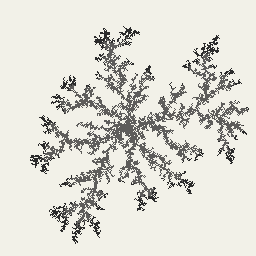
\includegraphics[width=\textwidth]{fig/colony_starved.png}
  \caption{$n_0=\num{0.10}$: starved}
\end{subfigure}\hfill
\begin{subfigure}[b]{0.29\textwidth}
  
\includegraphics[width=\textwidth]{fig/colony_fed.png}
  \caption{$n_0=\num{0.45}$: fed, at gen.\ 250}
\end{subfigure}\hfill
\begin{subfigure}[b]{0.40\textwidth}
\begin{tikzpicture}
\begin{axis}[
  width=6.2cm, height=5.2cm,
  xlabel={initial nutrient $n_0$}, ylabel={box dimension $D$},
  xmode=log, log basis x=10,
  ymin=1.3, ymax=2.1, grid=both,
  legend pos=south east,
]
\addplot[only marks, mark=*, mark size=1.4pt, ink]
  table[x=n0, y=D, col sep=comma] {data/colony_food.csv};
\addplot[dashed, warm, thick, domain=0.04:0.9] {2.0};
\addlegendentry{measured}
\addlegendentry{compact, $D=2$}
\addplot[dotted, accent, thick, domain=0.04:0.9] {1.71};
\addlegendentry{DLA, $D=1.71$}
\end{axis}
\end{tikzpicture}
\caption{$D$ against food}
\end{subfigure}
\caption{The colony's morphology is set by one environmental number. Nothing
about the cells is different between (a) and (b). $D$ falls monotonically as food
is withdrawn, crossing the diffusion-limited-aggregation value near
$n_0\approx\num{0.14}$ and reaching $D=\num{2.00}$ above $n_0\approx\num{0.40}$. The
fed colony (b) is caught at generation 250, while its growth front still exists:
left alone it reaches the walls of the dish by generation 450 and the picture
becomes a solid black square, which is true and shows nothing. What matters in (b)
is that the front is smooth and convex --- there are no fingers to see. Witten and
Sander derived $D=\num{1.71}$ for DLA from an
argument about random walkers with no biology in it \cite{witten1981}; Fujikawa
and Matsushita measured $D\approx\num{1.73}$ on a plate of \emph{Bacillus
subtilis} \cite{fujikawa1989}.}
\label{fig:colony}
\end{figure}

The two leftmost points of the curve should be read with care. Below
$n_0\approx\num{0.07}$ the colony never exceeds a few thousand cells, and box
counting on a cluster that small is biased downwards by the finite lattice: the
apparent $D=\num{1.42}$ at $n_0=\num{0.05}$ reflects the size of the object as
much as its geometry. The regime in which the estimate is trustworthy --- where
the cluster spans enough octaves for a scaling range to exist --- is roughly
$\num{0.10} \le n_0 \le \num{0.45}$, and it is across that range that the
dimension moves from fractal to compact.

It is worth being precise about the cause, because ``the colony branches because
it is hungry'' is not quite right. Branching requires the instability, and the
instability requires that the nutrient field around the colony relax into a
quasi-static harmonic field, so that tips see far more of it than hollows do.
That in turn requires a long \emph{diffusion length}: nutrient must travel a good
distance between one division and the next. Figure~\ref{fig:difflen} holds the
food fixed and varies only the diffusion length, and the morphology moves
anyway. Starve a colony but let it eat only what is immediately in front of it,
and it does not branch --- it starves compactly.

\begin{figure}[t]
\centering
\begin{tikzpicture}
\begin{axis}[
  width=11cm, height=5.4cm,
  xlabel={diffusion length $D_n \times \mathrm{substeps}$ (nutrient travel per division)},
  ylabel={box dimension $D$},
  grid=both, ymin=1.5, ymax=2.05,
]
\addplot[only marks, mark=*, mark size=1.3pt, ink]
  table[x=difflen, y=D, col sep=comma] {data/colony_difflen.csv};
\end{axis}
\end{tikzpicture}
\caption{Food held fixed at $n_0=\num{0.16}$; only the diffusion length varies.
The colony is equally hungry throughout. Branching is not caused by hunger; it is
caused by hunger \emph{plus} a diffusion field long enough for a tip to exploit.}
\label{fig:difflen}
\end{figure}

\subsection{Mild preferences, segregated cities}

Schelling's households look at their eight neighbours and move if fewer than a
fraction $\tau$ of them are of their own kind. A randomly mixed city of two equal
groups scores $\num{0.5}$ on the segregation index by chance. The system halts as
soon as every household is content, so $\tau$ does not merely influence the
outcome --- it \emph{sets} it, and the city segregates exactly as far as it must
and no further.

The result is the gap between the two axes of Figure~\ref{fig:schelling}. At
$\tau=\num{0.35}$ --- a population in which everyone is perfectly content to be
outnumbered nearly two to one, which is more tolerant than any society that has
ever existed --- the city still settles at a segregation index of
$\num{0.771}\pm\num{0.002}$, against a chance baseline of $\num{0.50}$. The curve
has already left the baseline by $\tau=\num{0.15}$ and is at $\num{0.93}$ by
$\tau=\num{0.50}$. There is no threshold of intolerance below which the city is
safe.

\begin{figure}[t]
\centering
\begin{tikzpicture}
\begin{axis}[
  width=11cm, height=5.4cm,
  xlabel={tolerance $\tau$ (fraction of like neighbours each household requires)},
  ylabel={segregation index},
  grid=both, ymin=0.45, ymax=1.0, xmin=0.02, xmax=0.83,
  legend pos=north west,
]
\addplot[dashed, ink!50, thick, domain=0.02:0.83] {0.5};
\addlegendentry{chance ($\num{0.50}$)}
\addplot[mark=*, mark size=1.4pt, ink, thick, error bars/.cd, y dir=both, y explicit]
  table[x=tau, y=segregation, y error=sd, col sep=comma] {data/schelling.csv};
\addlegendentry{measured (5 seeds)}
\end{axis}
\end{tikzpicture}
\caption{Segregation against tolerance, after 500 rounds on a $128^2$ lattice
with 15\% vacancy. The curve leaves the chance baseline long before $\tau=0.5$.
Nobody in this model prefers a segregated city; the city segregates regardless.}
\label{fig:schelling}
\end{figure}

\subsection{A fair world and an unfair distribution}

Sugarscape's rules are scrupulously fair: agents inherit nothing, cheat nobody,
and draw their vision, metabolism and starting endowment from the same
distributions. Figure~\ref{fig:sugar} shows the Gini coefficient of the wealth
distribution over time, from an initial condition in which everybody has roughly
the same. Two things emerge that nobody specified: a carrying capacity, and
inequality.

\begin{figure}[t]
\centering
\begin{subfigure}[b]{0.48\textwidth}
\begin{tikzpicture}
\begin{axis}[
  width=7.2cm, height=4.8cm,
  xlabel={generation}, ylabel={Gini coefficient},
  grid=both, ymin=0, ymax=0.55,
]
\addplot[ink, thick] table[x=t, y=gini, col sep=comma] {data/sugarscape.csv};
\end{axis}
\end{tikzpicture}
\caption{inequality}
\end{subfigure}\hfill
\begin{subfigure}[b]{0.48\textwidth}
\begin{tikzpicture}
\begin{axis}[
  width=7.2cm, height=4.8cm,
  xlabel={generation}, ylabel={population},
  grid=both, ymin=0,
]
\addplot[accent, thick] table[x=t, y=population, col sep=comma] {data/sugarscape.csv};
\end{axis}
\end{tikzpicture}
\caption{carrying capacity}
\end{subfigure}
\caption{Sugarscape, from an initial population of 400 with endowments drawn
uniformly from $[5,25]$. (a) The Gini coefficient of the wealth distribution
climbs away from equality within a few tens of generations, peaks at
$\num{0.434}$, and settles at $\num{0.40}$ --- which is roughly the Gini of a
real economy. Nothing in the rules distributes anything unfairly. (b) The
population overshoots, crashes, and settles at 214 agents: a carrying capacity
that is a property of the landscape and of nothing anybody decided.}
\label{fig:sugar}
\end{figure}

\subsection{Biodiversity as a phase transition}

Three species in a cycle where none is strongest. In a well-mixed system this
ends in a monoculture. On a lattice it need not --- and whether it does is
decided by a single number, the rate at which neighbours exchange places.
Reichenbach, Mobilia and Frey showed that below a critical mobility the system
organises into interlocking spiral waves and all three species persist
indefinitely; above it, the spiral wavelength (which grows as $\sqrt{M}$) exceeds
the system size, the pattern washes out, and biodiversity collapses
\cite{reichenbach2007}. Figure~\ref{fig:rps} reproduces the transition: on a
$128^2$ lattice, all three species survive every run up to $\epsilon=4$, and by
$\epsilon=55$ every run has collapsed to a monoculture, with the crossover near
$\epsilon\approx\num{18}$.

\begin{figure}[t]
\centering
\begin{subfigure}[b]{0.30\textwidth}
  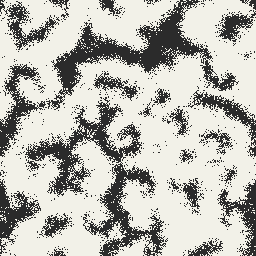
\includegraphics[width=\textwidth]{fig/rps_spirals.png}
  \caption{$\epsilon=2$: coexistence}
\end{subfigure}\hfill
\begin{subfigure}[b]{0.66\textwidth}
\begin{tikzpicture}
\begin{axis}[
  width=8.6cm, height=5.2cm,
  xlabel={exchange rate $\epsilon$ (mobility)},
  ylabel={P(extinction) after 1500 gen},
  xmode=log, grid=both, ymin=-0.05, ymax=1.05,
]
\addplot[mark=*, mark size=1.4pt, ink, thick]
  table[x=eps, y=extinction, col sep=comma] {data/rps.csv};
\end{axis}
\end{tikzpicture}
\caption{Extinction probability against mobility (8 seeds per point)}
\end{subfigure}
\caption{One slider takes the system from a living ecosystem to a monoculture.
The three strains are not a metaphor: Kerr \emph{et al.} played this game with
real \emph{E.\,coli}, and got the same answer --- in a flask one strain took
over, on a plate all three persisted \cite{kerr2002}.}
\label{fig:rps}
\end{figure}

\subsection{Classifying all 256 elementary rules}

Wolfram sorted the elementary rules into four classes by eye \cite{wolfram1983}.
Wuensche's input entropy does it mechanically and, more importantly,
\emph{quantitatively} \cite{wuensche1999}: at each step, take the Shannon entropy
of the histogram of how many cells matched each of the eight neighbourhood
patterns. Rules that freeze drive it low and flat; rules that boil hold it high
and flat; the interesting rules sit in between with a \emph{large variance},
because the entropy jerks around as coherent structures form, collide and die.
The variance of the input entropy is a glider detector.

Figure~\ref{fig:eca} places all 256 rules in that plane, and the statistic does
most of what it claims. The fully chaotic rules cluster at the right-hand edge:
rule 30 and rule 90 both sit at a mean entropy of $\approx\!\num{2.98}$ bits (of a
possible 3) with a variance of order $\num{1e-4}$, which is to say they boil
steadily and never stop boiling. Rules with intermediate entropy
($\num{2.7} < H < \num{2.95}$) have a median variance of $\num{4.1e-4}$, five
times that of the fully chaotic band ($\num{8e-5}$), and it is in this
intermediate band that the two rules Wolfram singles out as class IV are found:
rule 110, which Cook proved Turing complete \cite{cook2004}, at
$H=\num{2.907}$, $\mathrm{Var}=\num{4.3e-4}$, and rule 54 at $H=\num{2.908}$,
$\mathrm{Var}=\num{3.4e-3}$.

But we should be honest about what the statistic does \emph{not} do, because our
own figure shows it. The very highest variances in the plane do not belong to rule
110 at all; they belong to rules 1, 5 and 127, whose entropy simply oscillates
with period two because the whole lattice inverts every step. A variance is a
variance: it cannot tell an entropy that jumps because gliders are colliding from
an entropy that jumps because the pattern is blinking. What rescues the classifier
is the \emph{other} axis --- those rules sit at low mean entropy
($\num{1.5}$--$\num{1.7}$ bits) and are nowhere near the complex band --- so the
two coordinates together separate the classes even though neither does alone. It
is a good illustration of why one measures two things and plots them against each
other rather than reporting a single number.

\begin{figure}[t]
\centering
\begin{subfigure}[b]{0.62\textwidth}
\begin{tikzpicture}
\begin{axis}[
  width=8.4cm, height=5.8cm,
  xlabel={mean input entropy $H$ (bits)},
  ylabel={variance of input entropy},
  ymode=log, ymin=1e-6, ymax=1e-1,
  grid=both, legend pos=north west,
  legend style={font=\tiny},
]
\addplot[only marks, mark=*, mark size=0.9pt, ink!35]
  table[x=entropy, y=variance, col sep=comma] {data/eca.csv};
\addlegendentry{all 256 rules}
\addplot[only marks, mark=*, mark size=2.0pt, warm]
  table[x=entropy, y=variance, col sep=comma] {data/eca_notable.csv};
\addlegendentry{4, 30, 54, 90, 110, 184}
\node[font=\tiny, color=warm, anchor=south] at (axis cs:2.907,4.3e-4) {110};
\node[font=\tiny, color=warm, anchor=north] at (axis cs:2.908,3.4e-3) {54};
\node[font=\tiny, color=warm, anchor=west] at (axis cs:2.984,2.0e-4) {30};
\node[font=\tiny, color=warm, anchor=east] at (axis cs:2.986,1.1e-4) {90};
\end{axis}
\end{tikzpicture}
\caption{all 256 rules}
\end{subfigure}\hfill
\begin{subfigure}[b]{0.18\textwidth}
  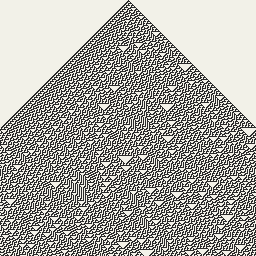
\includegraphics[width=\textwidth]{fig/eca_r30.png}
  \caption{rule 30}
\end{subfigure}\hfill
\begin{subfigure}[b]{0.18\textwidth}
  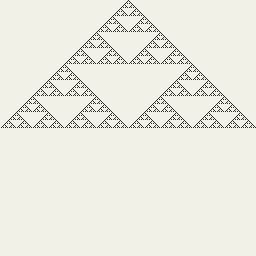
\includegraphics[width=\textwidth]{fig/eca_r90.png}
  \caption{rule 90}
\end{subfigure}
\caption{Automatic classification of the whole elementary rulespace (log
variance axis). Ordered rules collapse to the bottom left; the fully chaotic
rules --- rule 30 and rule 90 among them --- pile up at the right-hand edge with
a steady, high entropy and almost no variance in it. The class IV rules sit to
their left, at intermediate entropy and higher variance --- rule 54 by an order of
magnitude, rule 110 only by a factor of two, which is a thinner margin than the
method's reputation suggests. The outliers at the top left are not complex; they are rules whose
lattice inverts every step, so their entropy oscillates with period two --- which
is why the classifier needs both coordinates and not just the variance. Rule 90
(c), from a single live cell, is the Sierpi\'{n}ski triangle, and box-counts to
$D=\num{1.585}=\log 3/\log 2$.}
\label{fig:eca}
\end{figure}

\subsection{Lenia: the niche is a filament}

Lenia \cite{chan2019} dissolves every discrete feature of Conway's Life: the
state is real-valued, the neighbourhood is a smooth ring-shaped kernel, the birth
and survival sets become a smooth growth function, and the time step is small.

\begin{equation}
A_{t+\Delta t} = \bigl[\, A_t + \tfrac{1}{T}\, G(K * A_t) \,\bigr]_0^1,
\qquad
G(u) = 2\exp\!\left(-\frac{(u-\mu)^2}{2\sigma^2}\right) - 1 .
\end{equation}

What survives the dissolution is a creature. \emph{Orbium unicaudatus} holds its
shape, moves under its own power in a direction of its own choosing, and repairs
itself when damaged --- and it dies if the parameters leave a narrow region of
the $(\mu,\sigma)$ plane. Figure~\ref{fig:lenia} maps that region. It is a
filament. The claim that life sits at an ``edge'' between order and chaos is
usually made rhetorically; here it is a measurement, and the edge is about six
thousandths of $\sigma$ wide.

\begin{figure}[t]
\centering
\begin{subfigure}[b]{0.24\textwidth}
  
\includegraphics[width=\textwidth]{fig/lenia_orbium.png}
  \caption{Orbium}
\end{subfigure}\hfill
\begin{subfigure}[b]{0.72\textwidth}
\begin{tikzpicture}
\begin{axis}[
  width=9.6cm, height=5.4cm,
  xlabel={growth centre $\mu$}, ylabel={growth width $\sigma$},
  grid=both, point meta min=0, point meta max=1,
  colormap={ink}{color=(papergrey) color=(ink)},
]
\addplot[scatter, only marks, mark=square*, mark size=1.35pt,
         scatter src=explicit, point meta=explicit]
  table[x=mu, y=sigma, meta=alive, col sep=comma] {data/lenia.csv};
\end{axis}
\end{tikzpicture}
\caption{where Orbium survives 400 steps}
\end{subfigure}
\caption{Dark squares: the creature is still there, still bounded, still itself,
after 400 steps. Light: it either evaporated or bloomed into structureless mush
that fills the world. Both are deaths. Life occupies the filament between them.}
\label{fig:lenia}
\end{figure}

\subsection{Self-organised criticality, and what destroys it}

The Drossel--Schwabl forest fire \cite{drossel1992} needs no parameter tuned to a
critical value: given a wide separation between the growth rate $p$ and the
lightning rate $f$, the forest drives \emph{itself} to a critical density and
stays there, and fires arrive with no characteristic size.
Figure~\ref{fig:fire} shows the fire-size distribution in that regime and in one
where the separation of timescales has been destroyed. The power law is not a
property of the rules. It is a property of the rules \emph{plus} the separation
of timescales, and it disappears when the separation does.

\begin{figure}[t]
\centering
\begin{subfigure}[b]{0.30\textwidth}
  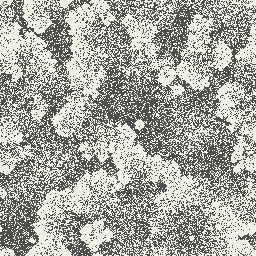
\includegraphics[width=\textwidth]{fig/forestfire.png}
  \caption{$f/p = 10^{-3}$}
\end{subfigure}\hfill
\begin{subfigure}[b]{0.66\textwidth}
\begin{tikzpicture}
\begin{axis}[
  width=8.6cm, height=5.4cm,
  xlabel={fire size $s$ (trees consumed)}, ylabel={count},
  xmode=log, ymode=log, grid=both, legend pos=north east,
]
\addplot[only marks, mark=*, mark size=1.5pt, ink]
  table[x=size, y=count, col sep=comma] {data/forestfire_critical.csv};
\addlegendentry{$f/p=10^{-3}$}
\addplot[only marks, mark=square, mark size=1.5pt, warm]
  table[x=size, y=count, col sep=comma] {data/forestfire_driven.csv};
\addlegendentry{$f/p=5\times10^{-2}$}
\end{axis}
\end{tikzpicture}
\caption{fire-size distribution}
\end{subfigure}
\caption{Fire sizes, binned by octave. The near-horizontal black distribution is
the signature, not a contradiction of it: with logarithmic bins, a power law
$P(s)\sim s^{-\tau}$ with $\tau\approx\num{1.15}$ gives a count per octave going
as $s^{1-\tau}=s^{-0.15}$, which is almost flat. Fires of every size occur with
comparable frequency across five decades, until the finite lattice cuts the tail
off. The red distribution, with lightning fifty times more frequent, has a scale:
it stops dead at a few hundred trees.}
\label{fig:fire}
\end{figure}

The two regimes are separated most sharply not by the number of fires but by
their extremes. Over \num{20000} generations on a $256^2$ lattice, the critical
regime ($p=\num{0.02}$, $f=\num{2e-5}$) produced \num{11008} fires, the largest
of which consumed \num{221702} trees --- many times the number standing at any
one moment, since the fire outran the regrowth across the entire lattice. The
driven regime ($f=\num{1e-3}$) produced forty times as many fires,
\num{442025} of them, and the largest consumed \num{1320}. Frequent lightning
does not make the forest more flammable. It makes it \emph{safe}, by never
letting it become connected enough to burn properly --- and in doing so it
abolishes the scale-free behaviour entirely.

\section{Validation}
\label{sec:validation}

The models are not checked against their own previous output. They are checked
against numbers that other people measured, several of them with actual bacteria.
These are assertions in \texttt{tests/main.c}, they run natively, and continuous
integration runs them on every push. When one of them drifts, it is a bug, not a
tolerance to be widened.

\begin{table}[h]
\centering
\small
\begin{tabular}{@{}llll@{}}
\toprule
\textbf{Model} & \textbf{Quantity} & \textbf{Expected} & \textbf{Source} \\
\midrule
Colony (starved) & box dimension & fractal, $\to 1.7$ & \cite{witten1981,fujikawa1989} \\
Colony (fed) & box dimension & $2.0$ (compact) & --- \\
ECA rule 90 & box dimension & $\log 3/\log 2 = 1.585$ & \cite{wolfram1983} \\
Life, random soup & ash density & $\approx 0.03$ & --- \\
Life, glider & cells after 64 gen & $5$ (and translated) & \cite{gardner1970} \\
Sugarscape & Gini from equal starts & $0.4$--$0.5$ & \cite{epstein1996} \\
Schelling, $\tau=0.35$ & segregation index & $\approx 0.77$ (chance: $0.50$) & \cite{schelling1971} \\
Schelling, $\tau=0.50$ & segregation index & $> 0.85$ & \cite{schelling1971} \\
Lenia, Orbium & mass after 400 steps & bounded, nonzero & \cite{chan2019} \\
Lenia, $\sigma=0.005$ & mass after 300 steps & zero (dies) & \cite{chan2019} \\
Cyclic competition & species at high mobility & $< 3$ (extinction) & \cite{reichenbach2007} \\
Forest fire & tree density & self-organises, $0.2 < \rho < 0.75$ & \cite{drossel1992} \\
All models & re-run from same seed & bit-identical & --- \\
\bottomrule
\end{tabular}
\caption{The literature, as a test suite.}
\end{table}

\section{Negative results}
\label{sec:negative}

The failures were more instructive than most of the successes, and three of them
generalise.

\paragraph{A fractal dimension in the right range is weak evidence.}
The first version of the colony model let its cells wander freely inside a
lubricated envelope, in the spirit of Ben-Jacob's communicating walkers. It
produced a diffuse cloud of live cells, and that cloud box-counted to
$D\approx\num{1.71}$ --- squarely on the Witten--Sander value, and squarely
wrong. A scattered point cloud is fractal too. The test passed; the physics was
absent. The model only started producing colonies when the cells were made
\emph{static}, so that the structure was a scaffold of spent cells with growth
confined to a thin living rind. We report this because the scalar was doing
exactly what a scalar does: it summarised, and in summarising it discarded the
distinction between a colony and a gas. We now look at the images as well, and we
recommend that anybody validating a growth model against $D$ alone does the same.

\paragraph{Surface diffusion is not surface tension without a coordination bias.}
We attempted a second morphological axis --- agar hardness, following Matsushita
--- implemented as surface diffusion: a newborn cell takes a few steps along the
colony's surface before settling. It did not smooth the interface. It merely
dumped daughters somewhere arbitrary, half of them in a starved crevice where
they died, so the colony grew more slowly and no rounder. Adding a preference for
sites of high coordination (more occupied neighbours, as an adatom prefers a kink
site) made the sliding smooth the interface, but at the cost of pulling daughters
\emph{inward}, which stalled the growth front entirely. We removed the axis rather
than ship a control that does not do what its label says. The paper and the
interface now claim only the axis we can demonstrate: the diffusion length
(Figure~\ref{fig:difflen}).

\paragraph{The obvious way to count a fire destroys the power law.}
In the forest fire, treating every cell burning anywhere on the map at a given
moment as one fire --- closing the books when the last ember goes out --- seems
harmless. It is fatal. In precisely the regime the model exists to study, two
independent fires are almost always burning somewhere at once, so the map is never
cold, so the counter never closes, and 1500 generations report a single enormous
fire. The power law, which is the entire point, vanishes. Each ignition must open
a numbered fire, and its number must be inherited by every tree it spreads to.

\paragraph{A note on Lenia's kernel.}
Chan's paper presents the exponential kernel core $\exp(4 - 1/(r(1-r)))$ and a
Gaussian growth function, and that is the form every secondhand description
repeats. The reference implementation defaults to the \emph{polynomial}
$(4r(1-r))^4$ and a polynomial growth function, and every creature in the species
list --- Orbium included --- was found under the polynomial. Loaded under the
exponential core, Orbium does not glide; it wobbles and dies. We ship both, with
the polynomial as the default, because that is the physics the animals actually
live in.

\section{Limitations and further work}

The most significant omission is a sweep engine: a worker pool that runs a model
headlessly across a parameter grid and renders the resulting phase diagram in the
browser, with a ``reproduce the figure'' button on each model that regenerates the
figure from its own source paper. The figures in this paper were produced exactly
this way, but natively, from \texttt{tools/figures.c}; exposing the same
capability interactively is the natural next step, and the architecture (a
portable core with no browser dependency) was chosen with it in mind.

Lenia's convolution is direct rather than FFT-based, which caps the practical
kernel radius. Cross-origin isolation is unavailable on GitHub Pages, so
\texttt{SharedArrayBuffer} and therefore WebAssembly threads are off the table;
the simulation runs on the main thread under a wall-clock budget. Neither is
fundamental.

\section{Conclusion}

A cellular automaton is worth taking seriously when you can measure it, argue with
it, and hand it to somebody else exactly as you found it. The models here are
small --- the whole simulation core is a few thousand lines of C, and it compiles
to 64\,KB of WebAssembly --- but they reproduce, from local rules and nothing
else, a fractal dimension that somebody obtained from a Petri dish, a wealth
distribution that nobody designed, a segregated city that nobody wanted, and a
creature that repairs itself.

\begin{thebibliography}{99}\small

\bibitem{bak1987} Bak, P., Tang, C. \& Wiesenfeld, K.
  Self-organized criticality: An explanation of $1/f$ noise.
  \emph{Phys. Rev. Lett.} \textbf{59}, 381--384 (1987).

\bibitem{benjacob1994} Ben-Jacob, E., Schochet, O., Tenenbaum, A., Cohen, I.,
  Czir\'{o}k, A. \& Vicsek, T.
  Generic modelling of cooperative growth patterns in bacterial colonies.
  \emph{Nature} \textbf{368}, 46--49 (1994).

\bibitem{chan2019} Chan, B. W.-C.
  Lenia --- Biology of Artificial Life.
  \emph{Complex Systems} \textbf{28}(3), 251--286 (2019). arXiv:1812.05433.

\bibitem{cook2004} Cook, M.
  Universality in Elementary Cellular Automata.
  \emph{Complex Systems} \textbf{15}, 1--40 (2004).

\bibitem{drossel1992} Drossel, B. \& Schwabl, F.
  Self-organized critical forest-fire model.
  \emph{Phys. Rev. Lett.} \textbf{69}, 1629--1632 (1992).

\bibitem{epstein1996} Epstein, J. M. \& Axtell, R.
  \emph{Growing Artificial Societies: Social Science from the Bottom Up.}
  Brookings Institution Press / MIT Press (1996).

\bibitem{fujikawa1989} Fujikawa, H. \& Matsushita, M.
  Fractal growth of \emph{Bacillus subtilis} on agar plates.
  \emph{J. Phys. Soc. Jpn.} \textbf{58}, 3875--3878 (1989).

\bibitem{gardner1970} Gardner, M.
  Mathematical Games: The fantastic combinations of John Conway's new solitaire
  game ``life''. \emph{Scientific American} \textbf{223}(4), 120--123 (1970).

\bibitem{kerr2002} Kerr, B., Riley, M. A., Feldman, M. W. \& Bohannan, B. J. M.
  Local dispersal promotes biodiversity in a real-life game of
  rock--paper--scissors. \emph{Nature} \textbf{418}, 171--174 (2002).

\bibitem{langton1986} Langton, C. G.
  Studying artificial life with cellular automata.
  \emph{Physica D} \textbf{22}, 120--149 (1986).

\bibitem{matsushita1998} Matsushita, M. \emph{et al.}
  Interface growth and pattern formation in bacterial colonies.
  \emph{Physica A} \textbf{249}, 517--524 (1998).

\bibitem{oneill2014pcg} O'Neill, M. E.
  PCG: A family of simple fast space-efficient statistically good algorithms for
  random number generation. Harvey Mudd College, HMC-CS-2014-0905 (2014).

\bibitem{pearson1993} Pearson, J. E.
  Complex patterns in a simple system.
  \emph{Science} \textbf{261}, 189--192 (1993).

\bibitem{reichenbach2007} Reichenbach, T., Mobilia, M. \& Frey, E.
  Mobility promotes and jeopardizes biodiversity in rock--paper--scissors games.
  \emph{Nature} \textbf{448}, 1046--1049 (2007).

\bibitem{schelling1971} Schelling, T. C.
  Dynamic models of segregation.
  \emph{J. Mathematical Sociology} \textbf{1}(2), 143--186 (1971).

\bibitem{turing1952} Turing, A. M.
  The chemical basis of morphogenesis.
  \emph{Phil. Trans. R. Soc. B} \textbf{237}, 37--72 (1952).

\bibitem{witten1981} Witten, T. A. \& Sander, L. M.
  Diffusion-limited aggregation, a kinetic critical phenomenon.
  \emph{Phys. Rev. Lett.} \textbf{47}, 1400--1403 (1981).

\bibitem{wolfram1983} Wolfram, S.
  Statistical mechanics of cellular automata.
  \emph{Rev. Mod. Phys.} \textbf{55}, 601--644 (1983).

\bibitem{wuensche1999} Wuensche, A.
  Classifying cellular automata automatically: finding gliders, filtering, and
  relating space-time patterns, attractor basins, and the Z parameter.
  \emph{Complexity} \textbf{4}(3), 47--66 (1999).

\end{thebibliography}

\end{document}
